\documentclass[report, backcover, french, nodocumentinfo]{upmethodology-document}
\usepackage[utf8]{inputenc}
\usepackage[T1]{fontenc}
%\usepackage{natbib}
\usepackage{csquotes}
%\usepackage[backend=biber,style=alphabetic,citestyle=authoryear]{biblatex}
\usepackage{amsmath}
\usepackage{amssymb}
\usepackage{hyperref}
\usepackage{listings}
\usepackage{textcomp}
\usepackage{color}
\usepackage[toc,page]{appendix}
\usepackage{wrapfig}
\usepackage{stackengine}
\usepackage{scalerel}

%link option, especialy for the table of contents
\hypersetup{
    colorlinks=true,
    linkcolor=black,
    urlcolor=blue,
    linktoc=all
}

\setfrontcover{classic}

\declaredocument{Conception de projet: clone de MiniMetro}{Rapport LO43}{LO43-A2016}
\setpublisher{Université de Technologie de Belfort-Montbéliard}

%\incversion{\makedate{jj}{mm}{aaaa}}{Initial version.}{\upmpublic}
\incversion{\today}{Initial version.}{\upmpublic}

\addauthorvalidator*[julien.barbier@utbm.fr]{Julien}{BARBIER}{Auteur original}
\addauthorvalidator*[maxime.pinard@utbm.fr]{Maxime}{PINARD}{Auteur original}

\addinformed*[franck.gechter@utbm.fr]{Franck}{GECHTER}{Professeur de l'UV LO43}

\setdockeywords{UTBM, LO43, MiniMetro, Java, JavaFX, UML}

\setcopyrighter{Julien BARBIER et Maxime PINARD}
\setpublisher{Julien BARBIER et Maxime PINARD}
\setprintingaddress{France}

%\setfrontcover{modern}
%\setfrontillustration[0.6]{figures/logo}

\graphicspath{./figures/}

%\bibsize{\normalfont}

\newcommand*\cleartoleftpage{%
  \clearpage
  \ifodd\value{page}\hbox{}\newpage\fi
}

\newcommand{\p}[1]{\paragraph{#1\\}}

%Function to print a warning sign
\newcommand{\dangersign}[1][2.5ex]
	{\renewcommand{\stacktype}{L}
		{\scaleto{\stackon[1pt]{\color{red}$\triangle$}{\fontsize{4pt}{4pt}\selectfont !}}{#1}}}

% For more information about UPmethodology: https://www.ctan.org/pkg/upmethodology

\begin{document}

	\pagenumbering{gobble}
	\upmdocumentsummary{}
	\upmdocumentauthors{}
	\upmdocumentinformedpeople{}

	\tableofcontents{}
	\listoffigures{}

	\chapter{sample chapter}
		\section{sample section}
			\subsection{sample subsection}
				\subsubsection{sample subsubsection}
					\paragraph*{sample paragraph}
						Lorem ipsum dolor sit amet, consectetur adipiscing elit. Quisque nec ante cursus, porttitor erat sit amet, egestas tortor. Nulla commodo eu diam in fermentum. Class aptent taciti sociosqu ad litora torquent per conubia nostra, per inceptos himenaeos. Vestibulum et lacus ultrices, gravida dolor laoreet, tincidunt purus. Nulla ut justo nec odio dictum vulputate. Proin vel nibh consequat, venenatis elit malesuada, commodo odio.
						\begin{figure}[h!]
							\centering
							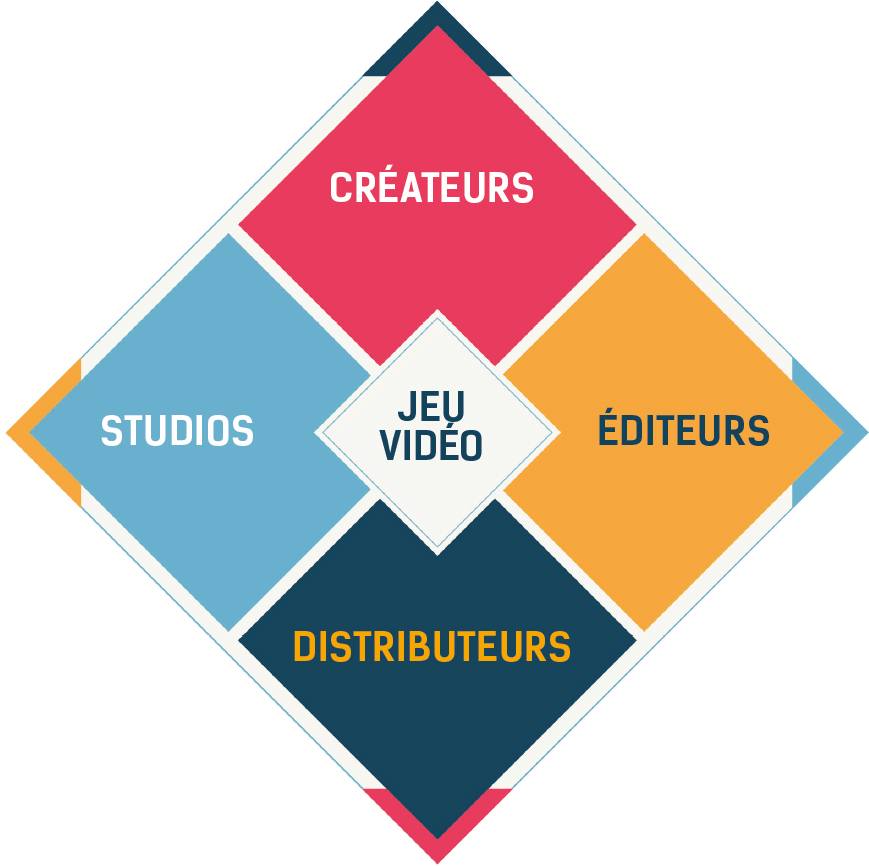
\includegraphics[width=0.5\textwidth]{figures/sample} % or <figures/sample.jpg>
							\caption{sample figure}
							\label{fig:sampleFigure}
						\end{figure}
					\p{}
						Lorem ipsum dolor sit amet, consectetur adipiscing elit. Quisque nec ante cursus, porttitor erat sit amet, egestas tortor. Nulla commodo eu diam in fermentum. Class aptent taciti sociosqu ad litora torquent per conubia nostra, per inceptos himenaeos. Vestibulum et lacus ultrices, gravida dolor laoreet, tincidunt purus. Nulla ut justo nec odio dictum vulputate. Proin vel nibh consequat, venenatis elit malesuada, commodo odio.
						sample text in anonymous paragraph
						\begin{upmcaution}
							This is an example of a caution message. This text must be rendered with enough height (usually 2 lines of text) to avoid intersection between the caution icon and the box frame.
						\end{upmcaution}
						\begin{upminfo}
							This is an example of an information message. This text must be rendered with enough height (usually 2 lines of text) to avoid intersection between the caution icon and the box frame.
						\end{upminfo}
						\begin{upmquestion}
							This is an example of a question message. This text must be rendered with enough height (usually 2 lines of text) to avoid intersection between the caution icon and the box frame.
						\end{upmquestion}
					\p{sample paragraph}
						footnote reference\footnote{sample footnote}\\
						\begin{emphbox}[.7\linewidth]
							This is an emphazed text.
						\end{emphbox}
	\chapter{sample chapter}
		\ldots
	%\theupmdockeywords
	%\makebackcover
\end{document}
